\documentclass[12pt]{article}

\pagestyle{empty}
\setlength{\topmargin}{0in}
\setlength{\headheight}{0in}
\setlength{\topsep}{0in}
\setlength{\textheight}{9in}
\setlength{\oddsidemargin}{0in}
\setlength{\evensidemargin}{0in}
\setlength{\textwidth}{6.5in}

\usepackage{palatino,graphics,amsmath}

\newcommand{\real}{{\bf R}}
\newcommand{\ds}{\displaystyle}
\begin{document}

\noindent
{\bf Mathematics 227} \\ 
{\bf Solutions to linear systems}

\bigskip
In this first exploration, we aim to develop some intuition for the
type of behavior we can expect to see when looking at solutions of
systems of linear equations.

\begin{enumerate}
\item We will first look at linear equations in two variables.
  \begin{itemize}
    \item On the plot below, graph the line $y=x+1$.  How many points
      satisfy this equation?
      \begin{center}
        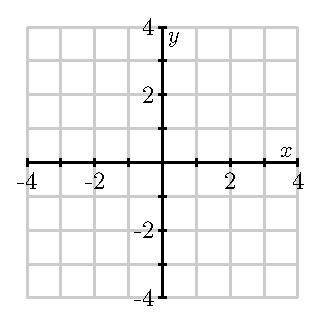
\includegraphics{empty-4.eps}
      \end{center}
    \item On the plot below, graph the lines
      $$
      \begin{aligned}
        y & = x + 1 \\
        y & = 2x - 1 \\
      \end{aligned}
      $$
      How many points satisfy both of these equations?
      \begin{center}
        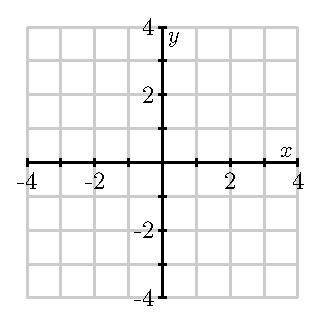
\includegraphics{empty-4.eps}
      \end{center}
    \item On the plot below, graph the lines
      $$
      \begin{aligned}
        y & = x + 1 \\
        y & = 2x - 1 \\
        y & = -x \\
      \end{aligned}
      $$
      How many points satisfy all of these equations?
      \begin{center}
        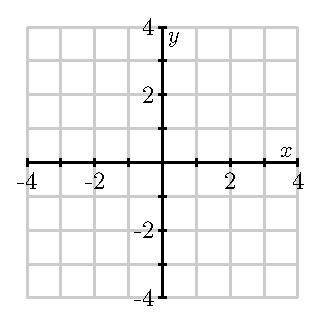
\includegraphics{empty-4.eps}
      \end{center}

    \item On the plot below, graph the lines
      $$
      \begin{aligned}
        y & = x + 1 \\
        y & = x - 1 \\
      \end{aligned}
      $$
      How many points satisfy both of these equations?
      \begin{center}
        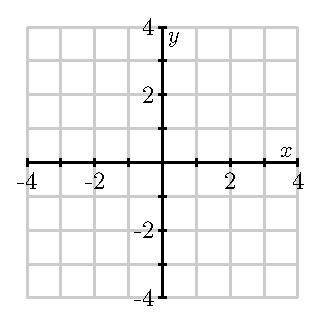
\includegraphics{empty-4.eps}
      \end{center}
    \item Based on what we've seen here, what are the possibilities for
      the solutions of a system of linear equations in two variables?
      
      \vspace{1in}
    \item What happens to the size of the solution sets as we add more
      equations? 
      
      \vspace{1in}
    \end{itemize}

    \newpage
  \item The solution to a linear equation in three variables $x$, $y$,
    and $z$ is a plane.  Use $3\times5$ cards to study the solutions
    to systems of linear equations in three variables.

    \begin{itemize}
      \item Is it possible that there are no solutions to a system of
        two equations in three variables?  If so, explain how or
        sketch an example.

        \vspace{1in}
      \item Is it possible that the solutions to a system of two
        equations in three variables is a single point?  If so,
        explain how or sketch an example.

        \vspace{1in}
      \item If you are studying a system of two equations in three
        variables, what would you usually expect for the solution set?

        \vspace{1in}
      \item If you are studying a system of three equations in three
        variables, what would you usually expect for the solution set?

        \vspace{1in}
      \item If you are studying a system of four equations in three
        variables, what would you usually expect for the solution
        set?

        \vspace{1in}
        \newpage
      \item Is it possible that four equations in three variables form
        a line?  If how, explain how or sketch an example.

        \vspace{1in}
      \item Is it possible that four equations in three variables form
        a plane?  If how, explain how or sketch an example.

      \vspace{1in}
      \item Based on what we've seen here, what are the possibilities for
      the solutions of a system of linear equations in three variables?
      
      \vspace{1in}
    \item What happens to the size of the solution sets as we add more
      equations? 
      
      \vspace{1in}
    \end{itemize}


\end{enumerate}



\end{document}
